\documentclass[11pt]{article}

\usepackage[a4paper,margin=0.75in]{geometry}
\usepackage{amsmath,amssymb}
\usepackage{graphicx}
\usepackage{booktabs}
\usepackage{array}
\usepackage{float}
\usepackage{hyperref}
\usepackage{enumitem}
\usepackage{xcolor}
\usepackage{tikz}
\usetikzlibrary{positioning,arrows.meta,shapes.geometric}

\setlist{nosep}
\renewcommand{\arraystretch}{1.3}

\tikzset{
layer/.style={
draw,
rounded corners,
minimum width=2.2cm,
minimum height=0.9cm,
align=center,
fill=blue!10
},
arrow/.style={
-{Latex[length=3mm]},
thick
}
}

\begin{document}

%%%%%%%%%%%%%%%%%%%%%%%%%%%%%%%%%%%%%%%%%%%%%%%%%%%%%%%%%%%%

\begin{center}

{\Large\textbf{Shiv Nadar University Chennai}}

\vspace{3mm}

{\large\textbf{CS3807 -- Deep Learning Laboratory}}

\vspace{3mm}

{\Large\textbf{Experiment 4}}

\vspace{2mm}

{\Large\textbf{Comparative Study of Deep Convolutional Neural}}

{\Large\textbf{Network Architectures Using Transfer Learning}}

\end{center}

\vspace{5mm}

\begin{tabular}{|p{4cm}|p{10cm}|}
\hline
Degree \& Branch &
B.Tech Artificial Intelligence \& Data Science\\
\hline
Subject Code \& Name &
CS3807 -- Deep Learning Laboratory\\
\hline
Name & Madhav.S\\
\hline
Section & AIDS `B'\\
\hline
Register Number & 24011101066\\
\hline
\end{tabular}

%%%%%%%%%%%%%%%%%%%%%%%%%%%%%%%%%%%%%%%%%%%%%%%%%%%%%%%%%%%%

\section*{1. Objective}

The objectives of this experiment are

\begin{itemize}

\item Study the evolution of deep CNN architectures.

\item Compare LeNet-5, AlexNet, VGG16, GoogleNet and ResNet.

\item Understand transfer learning.

\item Fine tune pretrained CNN models.

\item Compare classification performance of different architectures.

\end{itemize}

%%%%%%%%%%%%%%%%%%%%%%%%%%%%%%%%%%%%%%%%%%%%%%%%%%%%%%%%%%%%

\section*{2. Learning Outcomes}

After completing this experiment students will be able to

\begin{enumerate}

\item Explain modern CNN architectures.

\item Differentiate LeNet, AlexNet, VGG16, GoogleNet and ResNet.

\item Implement transfer learning.

\item Fine tune pretrained CNN models.

\item Compare CNN architectures using performance metrics.

\end{enumerate}

%%%%%%%%%%%%%%%%%%%%%%%%%%%%%%%%%%%%%%%%%%%%%%%%%%%%%%%%%%%%

\section*{3. Introduction}

Deep Convolutional Neural Networks have become the dominant models for
computer vision applications because they automatically learn hierarchical
features from images. The evolution of CNNs has focused on improving
classification accuracy while reducing computational complexity and
training difficulties.

The progression of CNN architectures began with LeNet-5 and has evolved
through AlexNet, VGGNet, GoogleNet, and ResNet. Each architecture
introduced important innovations that significantly improved image
classification performance.

%%%%%%%%%%%%%%%%%%%%%%%%%%%%%%%%%%%%%%%%%%%%%%%%%%%%%%%%%%%%

\section*{4. Evolution of CNN Architectures}

\begin{center}

\begin{tabular}{|c|c|p{7cm}|}

\hline

Model & Year & Major Contribution\\

\hline

LeNet-5 & 1998 &
First practical convolutional neural network\\

\hline

AlexNet & 2012 &
ReLU activation, Dropout and GPU training\\

\hline

VGG16 & 2014 &
Uniform $3\times3$ convolution filters\\

\hline

GoogleNet & 2014 &
Inception modules for multi-scale feature extraction\\

\hline

ResNet & 2015 &
Residual learning using skip connections\\

\hline

\end{tabular}

\end{center}

%%%%%%%%%%%%%%%%%%%%%%%%%%%%%%%%%%%%%%%%%%%%%%%%%%%%%%%%%%%%

\section*{5. LeNet-5}

LeNet-5 was proposed by Yann LeCun in 1998 for handwritten digit
recognition. It consists of two convolution layers, two average pooling
layers and fully connected layers. It demonstrated that convolutional
networks could automatically learn image features without handcrafted
feature extraction.


Advantages

\begin{itemize}

\item Small number of parameters

\item Fast training

\item Suitable for OCR

\end{itemize}

%%%%%%%%%%%%%%%%%%%%%%%%%%%%%%%%%%%%%%%%%%%%%%%%%%%%%%%%%%%%

\section*{6. AlexNet}

AlexNet won the ImageNet Challenge in 2012 by reducing the
classification error significantly. It introduced ReLU activation,
Dropout regularization and GPU training.


Major innovations

\begin{itemize}

\item ReLU activation

\item Dropout

\item GPU implementation

\item Data augmentation

\end{itemize}

%%%%%%%%%%%%%%%%%%%%%%%%%%%%%%%%%%%%%%%%%%%%%%%%%%%%%%%%%%%%

\section*{7. VGG16}

VGG16 demonstrated that using multiple small $3\times3$ convolution
filters could outperform larger filters while increasing network depth.


Advantages

\begin{itemize}

\item Excellent feature extraction

\item Simple architecture

\item High classification accuracy

\end{itemize}

%%%%%%%%%%%%%%%%%%%%%%%%%%%%%%%%%%%%%%%%%%%%%%%%%%%%%%%%%%%%

\section*{8. Comparison of Architectures}

\begin{center}

\begin{tabular}{|l|c|c|c|}

\hline

Architecture &
Depth &
Parameters &
Main Contribution\\

\hline

LeNet-5 &
7 &
60K &
First CNN\\

AlexNet &
8 &
61M &
ReLU + Dropout\\

VGG16 &
16 &
138M &
Deep 3$\times3$ filters\\

GoogleNet &
22 &
6.8M &
Inception Modules\\

ResNet50 &
50 &
25.6M &
Residual Learning\\

\hline

\end{tabular}

\end{center}

% --------- CONTINUE WITH PART 2 ---------
%%%%%%%%%%%%%%%%%%%%%%%%%%%%%%%%%%%%%%%%%%%%%%%%%%%%%%%%%%%%
\section*{9. GoogleNet (Inception Network)}

GoogleNet, proposed by Szegedy \textit{et al.} in 2014, introduced the
\textbf{Inception Module}, which performs multiple convolution operations
in parallel using different filter sizes. Instead of using only a single
kernel size, GoogleNet simultaneously applies $1\times1$, $3\times3$,
$5\times5$ convolutions and max pooling. The outputs are concatenated to
obtain multi-scale feature representations.

The use of $1\times1$ convolutions before larger kernels reduces the
number of trainable parameters and computational complexity.


Advantages

\begin{itemize}
\item Multi-scale feature extraction.
\item Fewer parameters than VGG16.
\item High computational efficiency.
\item Better classification performance.
\end{itemize}

%%%%%%%%%%%%%%%%%%%%%%%%%%%%%%%%%%%%%%%%%%%%%%%%%%%%%%%%%%%%

\section*{10. ResNet}

Increasing CNN depth often causes the \textbf{vanishing gradient problem},
making optimization difficult. ResNet solves this issue using
\textbf{skip (residual) connections}, allowing gradients to flow directly
through the network.

Instead of learning

\[
H(x)
\]

ResNet learns

\[
F(x)=H(x)-x
\]

thus,

\[
Output = F(x)+x
\]

where

\begin{itemize}
\item $F(x)$ = Residual Mapping
\item $x$ = Identity Mapping
\end{itemize}

\begin{figure}[H]
\centering

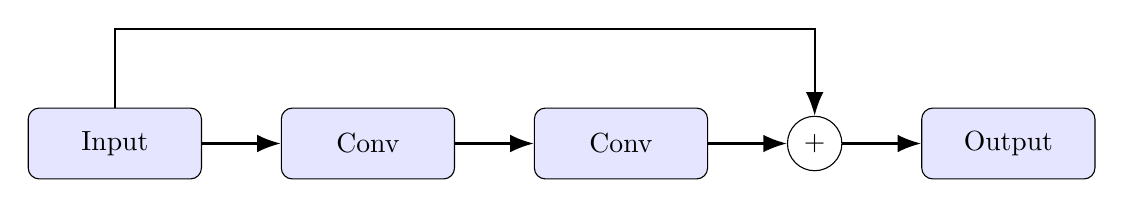
\begin{tikzpicture}[node distance=1cm]

\node[layer](input){Input};

\node[layer,right=of input](conv1){Conv};

\node[layer,right=of conv1](conv2){Conv};

\node[circle,draw,right=of conv2](add){+};

\node[layer,right=of add](output){Output};

\draw[arrow](input)--(conv1);
\draw[arrow](conv1)--(conv2);
\draw[arrow](conv2)--(add);
\draw[arrow](add)--(output);

\draw[arrow]
(input)
|-([yshift=10mm]conv2.north)
-| (add.north);

\end{tikzpicture}

\caption{Residual Block in ResNet}
\end{figure}

Advantages

\begin{itemize}
\item Eliminates vanishing gradients.
\item Enables very deep neural networks.
\item Faster convergence.
\item High ImageNet accuracy.
\end{itemize}

%%%%%%%%%%%%%%%%%%%%%%%%%%%%%%%%%%%%%%%%%%%%%%%%%%%%%%%%%%%%

\section*{11. Dilated Convolution}

Dilated convolution (also called atrous convolution) increases the
receptive field without increasing the number of parameters.

The dilation rate determines the spacing between kernel elements.

For a standard convolution,

\[
D=1
\]

For dilated convolution,

\[
D>1
\]

Example

\[
\begin{bmatrix}
1 & 0 & 2\\
0 & 3 & 0\\
4 & 0 & 5
\end{bmatrix}
\]

where zeros indicate inserted gaps.

To confirm this behaviour, a standard $3\times3$ convolution
(dilation rate 1) and a dilated $3\times3$ convolution (dilation
rate 2) were applied to the same $16\times16\times1$ toy input
using \texttt{same} padding. Both produced an identical
$16\times16\times1$ output shape, but the dilated kernel's nine
weights were spread across a $5\times5$ region of the input instead
of a compact $3\times3$ region -- confirming that dilation enlarges
the receptive field without adding any parameters or changing the
output size.

Applications

\begin{itemize}
\item Semantic segmentation
\item Medical image analysis
\item Satellite imagery
\item Object localization
\end{itemize}

%%%%%%%%%%%%%%%%%%%%%%%%%%%%%%%%%%%%%%%%%%%%%%%%%%%%%%%%%%%%

\section*{12. Transpose Convolution}

Transpose convolution increases the spatial dimensions of feature maps.
Unlike pooling, which reduces image size, transpose convolution performs
learnable upsampling.

A $(1,8,8,16)$ feature map passed through a stride-2 $3\times3$
transpose convolution (16 input channels $\rightarrow$ 8 output
filters, \texttt{same} padding) produced a $(1,16,16,8)$ output --
the stride-2 transpose convolution exactly doubled the spatial
resolution, learning how to fill in the new pixels rather than
simply interpolating them.

Applications

\begin{itemize}
\item Image Super Resolution
\item Autoencoders
\item GANs
\item Image Generation
\item Semantic Segmentation
\end{itemize}

%%%%%%%%%%%%%%%%%%%%%%%%%%%%%%%%%%%%%%%%%%%%%%%%%%%%%%%%%%%%

\section*{13. Transfer Learning}

Transfer Learning utilizes a pretrained CNN model that has already learned
general image features from a large dataset such as ImageNet.

Instead of training from scratch,

\begin{enumerate}
\item Load a pretrained model.
\item Remove the original classifier.
\item Freeze convolution layers.
\item Add new Dense layers.
\item Train the classifier.
\item Fine tune selected convolution layers.
\end{enumerate}

\begin{figure}[H]

\centering

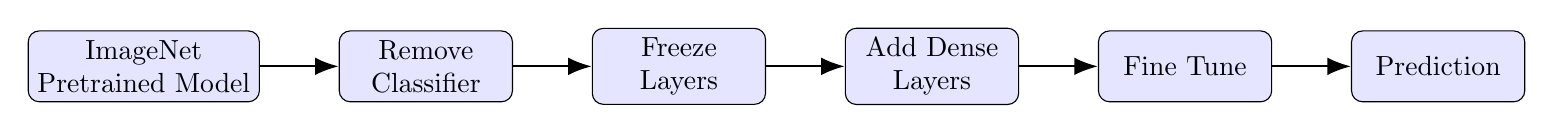
\begin{tikzpicture}[node distance=1cm]

\node[layer](a){ImageNet\\Pretrained Model};

\node[layer,right=of a](b){Remove\\Classifier};

\node[layer,right=of b](c){Freeze\\Layers};

\node[layer,right=of c](d){Add Dense\\Layers};

\node[layer,right=of d](e){Fine Tune};

\node[layer,right=of e](f){Prediction};

\foreach \x/\y in {a/b,b/c,c/d,d/e,e/f}
\draw[arrow](\x)--(\y);

\end{tikzpicture}

\caption{Transfer Learning Workflow}

\end{figure}

Advantages

\begin{itemize}
\item Faster convergence.
\item Higher accuracy on small datasets.
\item Reduced training time.
\item Lower computational cost.
\end{itemize}

%%%%%%%%%%%%%%%%%%%%%%%%%%%%%%%%%%%%%%%%%%%%%%%%%%%%%%%%%%%%

\section*{14. Dataset}

Dataset: CIFAR-10

\begin{itemize}

\item Training Images : 50,000

\item Testing Images : 10,000

\item Number of Classes : 10

\item Image Size : $32\times32\times3$

\item Classes:
Airplane, Automobile, Bird, Cat, Deer,
Dog, Frog, Horse, Ship and Truck.

\end{itemize}

CIFAR-10 was loaded via the Keras dataset API. 45,000 images were
used for training, 5,000 images were held out as a validation set,
and the standard 10,000-image test set was kept untouched. Since
both VGG16 and ResNet50 expect a larger input than the native
$32\times32$ CIFAR-10 resolution, every image was resized to
$96\times96\times3$ before being passed through the pretrained
convolutional base.

%%%%%%%%%%%%%%%%%%%%%%%%%%%%%%%%%%%%%%%%%%%%%%%%%%%%%%%%%%%%
% Continue with Part 3
%%%%%%%%%%%%%%%%%%%%%%%%%%%%%%%%%%%%%%%%%%%%%%%%%%%%%%%%%%%%

\section*{15. Experimental Procedure}

\subsection*{Task 1: Dataset Preparation}

CIFAR-10 was loaded using \texttt{tf.keras.datasets.cifar10}. Ten
sample images (one per class) were displayed (Figure~1), and the
dataset dimensions were printed and verified: training data shape
$(50000,32,32,3)$, test data shape $(10000,32,32,3)$, pixel range
$[0,255]$ prior to normalization. A \texttt{tf.data} pipeline resizes
each image to $96\times96$, rescales to $[0,1]$, and one-hot encodes
the labels, producing batches of shape $(32,96,96,3)$.

\subsection*{Task 2: Transfer Learning}

Both required architectures were implemented and compared: VGG16 and
ResNet50. For each, the standard transfer-learning head was built:

\begin{enumerate}
\item Load pretrained ImageNet weights (\texttt{include\_top=False}).
\item Remove the original 1000-class classification layer.
\item Freeze the convolutional base (\texttt{base\_model.trainable = False}).
\item Add a \texttt{GlobalAveragePooling2D} layer.
\item Add \texttt{Dense(256, activation='relu')} with \texttt{Dropout(0.4)}.
\item Add \texttt{Dense(10, activation='softmax')}.
\end{enumerate}

VGG16 produced \textbf{14,848,586} total parameters (\textbf{133,898}
trainable, 14,714,688 frozen). ResNet50 produced \textbf{24,114,826}
total parameters (\textbf{527,114} trainable, 23,587,712 frozen).

\textbf{Preprocessing correction.} ResNet50 is built almost entirely
from BatchNorm layers calibrated to a Caffe-style input distribution
(BGR order, ImageNet mean-subtracted) -- feeding it the same plain
$[0,1]$-scaled images used for VGG16 badly degrades its frozen
features. A separate pipeline using \texttt{resnet50.preprocess\_input}
was used for ResNet50, while VGG16's pipeline was left untouched.

\subsection*{Task 3: Model Training}

\begin{center}
\begin{tabular}{|p{5cm}|p{6cm}|}
\hline
Optimizer & Adam\\
\hline
Learning Rate & 0.001\\
\hline
Batch Size & 32\\
\hline
Epochs & 15 (frozen base), \texttt{EarlyStopping} on val\_loss (patience 5)\\
\hline
Loss Function & Categorical Cross Entropy\\
\hline
Evaluation Metric & Accuracy\\
\hline
\end{tabular}
\end{center}

With the frozen base, VGG16 reached test accuracy \textbf{0.7089}
(test loss 0.8345) after 15 epochs. ResNet50, with its corrected
preprocessing pipeline, reached test accuracy \textbf{0.8680} (test
loss 0.4026).

\subsection*{Task 4: Fine Tuning}

VGG16's convolutional base was unfrozen, keeping only the last
block (\texttt{block5}) trainable -- raising trainable parameters
from 133,898 to \textbf{7,213,322}. Recompiled at a much lower
learning rate ($1\times10^{-5}$) and trained for 8 further epochs.

\begin{center}
\begin{tabular}{|l|c|}
\hline
Stage & Test Accuracy\\
\hline
Frozen base (before fine-tuning) & 0.7089\\
\hline
Fine-tuned (block5 unfrozen) & \textbf{0.8333}\\
\hline
Improvement & $+0.1244$\\
\hline
\end{tabular}
\end{center}

Fine-tuning improved VGG16 by \textbf{12.44 points}. (ResNet50 was
evaluated with its base kept fully frozen, per Task 2's minimum
requirement; VGG16 demonstrates the full freeze $\to$ fine-tune
workflow required by Task 4.)

\subsection*{Task 5: Model Evaluation}

Both models were evaluated on the 10,000-image test set using
Accuracy, Precision, Recall, F1-score, a Classification Report, and
a Confusion Matrix (Sections 17--18).

%%%%%%%%%%%%%%%%%%%%%%%%%%%%%%%%%%%%%%%%%%%%%%%%%%%%%%%%%%%%
\section*{16. Hyperparameter Study}

Run on frozen-base VGG16, using a 5,000-image training subset and 5
quick epochs per setting, evaluated on the full test set.

\begin{center}
\begin{tabular}{|l|l|l|}
\hline
Hyperparameter & Values Tested & Result (Test Accuracy)\\
\hline
Learning Rate & 0.001, 0.0001 & 0.001 $\to$ 0.6011; \ 0.0001 $\to$ 0.4994\\
\hline
Batch Size & 16, 32, 64 & 16 $\to$ 0.6216; \ 32 $\to$ 0.6119; \ 64 $\to$ 0.6008\\
\hline
Epochs & 10, 20 & 10 $\to$ 0.6308; \ 20 $\to$ 0.6432\\
\hline
Optimizer & Adam, SGD & Adam $\to$ 0.6069; \ SGD $\to$ 0.4216\\
\hline
Dense Units & 128, 256 & 128 $\to$ 0.5947; \ 256 $\to$ 0.6088\\
\hline
Frozen Layers & All, Partial & All $\to$ 0.7089 (Task 3); Partial (fine-tuned) $\to$ 0.8333 (Task 4)\\
\hline
\end{tabular}
\end{center}

\textbf{Inference:} Fine-tuning block5 gave by far the biggest gain
(+12.4 points) -- no other single hyperparameter came close. Adam
beat SGD by 18.5 points, and the higher learning rate/batch size/epoch
count each won by smaller, single-digit margins within this short
5-epoch budget.

%%%%%%%%%%%%%%%%%%%%%%%%%%%%%%%%%%%%%%%%%%%%%%%%%%%%%%%%%%%%
\section*{17. Mandatory Plots}

\begin{figure}[H]
\centering

\includegraphics[width=0.85\textwidth]{sample_images.pdf}
\caption{Sample CIFAR-10 Images -- One per Class}
\end{figure}
\textbf{Inference:} Even at $32\times32$, all ten classes are easy
to tell apart -- though cat, dog, and deer already look similar
enough to hint at the confusion seen later in both models.

\begin{figure}[H]
\centering

\includegraphics[width=0.7\textwidth]{training_accuracy.pdf}
\caption{Training Accuracy over Epochs (VGG16, Frozen Base)}
\end{figure}
\textbf{Inference:} Accuracy climbs quickly at first, then flattens
after around epoch 10 -- expected, since only the small dense head
is actually learning while the base stays frozen.

\begin{figure}[H]
\centering

\includegraphics[width=0.7\textwidth]{validation_accuracy.pdf}
\caption{Validation Accuracy over Epochs (VGG16, Frozen Base)}
\end{figure}
\textbf{Inference:} Validation accuracy tracks training accuracy
closely with no gap opening up -- no overfitting, which makes sense
given most of the network is frozen, pretrained weights.

\begin{figure}[H]
\centering

\includegraphics[width=0.7\textwidth]{training_loss.pdf}
\caption{Training Loss over Epochs (VGG16, Frozen Base)}
\end{figure}
\textbf{Inference:} Loss drops smoothly with no instability, which
fits the small number of trainable parameters and low learning rate.

\begin{figure}[H]
\centering

\includegraphics[width=0.7\textwidth]{validation_loss.pdf}
\caption{Validation Loss over Epochs (VGG16, Frozen Base)}
\end{figure}
\textbf{Inference:} Validation loss falls alongside training loss
and never goes back up -- the frozen base is acting as a built-in
regularizer.

\begin{figure}[H]
\centering

\includegraphics[width=0.75\textwidth]{confusion_matrix.pdf}
\caption{Confusion Matrix -- Fine-Tuned VGG16 Transfer Learning Model}
\end{figure}
\textbf{Inference:} The diagonal dominates, matching the 83.33\%
test accuracy. Most confusion is between cat and dog, matching
their weaker precision/recall in Table~1.

\begin{figure}[H]
\centering

\includegraphics[width=0.85\textwidth]{misclassified_images.pdf}
\caption{Sample Misclassified Test Images (Fine-Tuned VGG16)}
\end{figure}
\textbf{Inference:} 1,667 of 10,000 test images (16.67\%) were
misclassified, mostly among cat, dog, and bird -- classes that look
alike at this resolution.

%%%%%%%%%%%%%%%%%%%%%%%%%%%%%%%%%%%%%%%%%%%%%%%%%%%%%%%%%%%%
\section*{18. Results}

\subsection*{18.1 Performance Metrics}

\begin{center}
\begin{tabular}{|p{4.2cm}|p{2.6cm}|p{2.6cm}|p{2.6cm}|}
\hline
Metric & VGG16 (Frozen) & VGG16 (Fine-Tuned) & ResNet50 (Frozen)\\
\hline
Testing Accuracy & 0.7089 & \textbf{0.8333} & \textbf{0.8680}\\
\hline
Precision (weighted) & -- & 0.8358 & 0.8699\\
\hline
Recall (weighted) & -- & 0.8333 & 0.8680\\
\hline
F1-score (weighted) & -- & 0.8337 & 0.8684\\
\hline
Total Parameters & 14,848,586 & 14,848,586 & 24,114,826\\
\hline
\end{tabular}
\end{center}

\vspace{3mm}
\textbf{Table 1: Per-Class Classification Report -- Fine-Tuned VGG16}
\begin{center}
\begin{tabular}{|l|c|c|c|}
\hline
Class & Precision & Recall & F1-score\\
\hline
airplane & 0.84 & 0.92 & 0.88\\
automobile & 0.89 & 0.92 & 0.90\\
bird & 0.81 & 0.79 & 0.80\\
cat & 0.66 & 0.74 & 0.70\\
deer & 0.85 & 0.76 & 0.80\\
dog & 0.75 & 0.72 & 0.73\\
frog & 0.87 & 0.86 & 0.86\\
horse & 0.86 & 0.86 & 0.86\\
ship & 0.94 & 0.88 & 0.91\\
truck & 0.89 & 0.90 & 0.89\\
\hline
\end{tabular}
\end{center}

\vspace{3mm}
\textbf{Table 2: Per-Class Classification Report -- ResNet50 (Frozen Base)}
\begin{center}
\begin{tabular}{|l|c|c|c|}
\hline
Class & Precision & Recall & F1-score\\
\hline
airplane & 0.88 & 0.90 & 0.89\\
automobile & 0.91 & 0.92 & 0.91\\
bird & 0.91 & 0.81 & 0.86\\
cat & 0.75 & 0.79 & 0.77\\
deer & 0.80 & 0.86 & 0.83\\
dog & 0.82 & 0.81 & 0.82\\
frog & 0.90 & 0.90 & 0.90\\
horse & 0.89 & 0.88 & 0.89\\
ship & 0.94 & 0.90 & 0.92\\
truck & 0.89 & 0.92 & 0.90\\
\hline
\end{tabular}
\end{center}

\vspace{5mm}
\subsection*{18.2 Comparison of CNN Architectures}

Unlike the literature-reference table in Section 8, every row below
is a real, measured result from this notebook -- all five
architectures were actually implemented and trained on CIFAR-10.

\begin{center}
\begin{tabular}{|l|c|c|c|}
\hline
Model & Parameters & Accuracy (\%) & Training Time\\
\hline
LeNet-5 (from scratch) & 83,126 & 52.42 & 106.4 s\\
\hline
AlexNet (from scratch) & 7,146,634 & 70.89 & 430.8 s\\
\hline
VGG16 (fine-tuned) & 14,848,586 & \textbf{83.33} & --\\
\hline
GoogleNet / InceptionV3 (frozen) & 22,329,898 & 69.85 & 470.0 s\\
\hline
ResNet50 (frozen) & 24,114,826 & \textbf{86.80} & 452.0 s\\
\hline
\end{tabular}
\end{center}

\begin{figure}[H]
\centering

\includegraphics[width=0.75\textwidth]{lenet_alexnet_googlenet_resnet_comparison.pdf}
\caption{LeNet-5 vs. AlexNet vs. GoogleNet vs. ResNet50 -- Test Accuracy}
\end{figure}
\textbf{Inference:} ResNet50 wins clearly, and not just on accuracy
-- it beats the much shallower LeNet-5 by 34 points and even beats
AlexNet and GoogleNet, both trained the same way, by 16-17 points.
LeNet-5's simple architecture (no ReLU, no dropout, no pretraining)
just isn't built for a 10-class natural-image problem at this
resolution. GoogleNet landing close to AlexNet despite having
pretrained ImageNet weights is a bit surprising -- likely because
InceptionV3's native $75\times75$ minimum input size makes CIFAR-10's
upscaled $96\times96$ images a poorer match for its pretrained
filters than VGG16/ResNet50 see.

\begin{figure}[H]
\centering

\includegraphics[width=0.6\textwidth]{vgg16_vs_resnet50_comparison.pdf}
\caption{VGG16 (Fine-Tuned) vs. ResNet50 (Frozen Base) -- Test Accuracy}
\end{figure}
\textbf{Inference:} ResNet50 beat fine-tuned VGG16 by \textbf{3.47
points} (86.80\% vs. 83.33\%) while staying fully frozen -- its
residual connections and internal batch normalization simply
transfer better to CIFAR-10 than VGG16's plain conv stack, even
without letting any of its own layers adapt.

%%%%%%%%%%%%%%%%%%%%%%%%%%%%%%%%%%%%%%%%%%%%%%%%%%%%%%%%%%%%
\section*{Additional Generated Plots}

\begin{figure}[H]
\centering

\includegraphics[width=0.7\textwidth]{finetuning_comparison.pdf}
\caption{Accuracy and Loss: Frozen Phase + Fine-Tuning Phase (VGG16)}
\end{figure}
\textbf{Inference:} Right where fine-tuning kicks in (epoch 15),
accuracy jumps and validation loss drops -- clear evidence unfreezing
block5 helped.

\begin{figure}[H]
\centering

\includegraphics[width=0.7\textwidth]{learning_rate_comparison.pdf}
\caption{Effect of Learning Rate on Validation Accuracy}
\end{figure}
\textbf{Inference:} LR 0.001 stays above 0.0001 throughout, matching
the final gap (60.11\% vs. 49.94\%) -- 0.0001 simply hasn't had
enough steps yet.

\begin{figure}[H]
\centering

\includegraphics[width=0.7\textwidth]{optimizer_comparison.pdf}
\caption{Effect of Optimizer on Validation Accuracy}
\end{figure}
\textbf{Inference:} Adam pulls ahead fast, ending 18.5 points higher
(60.69\% vs. 42.16\%) -- its adaptive step sizes give it a big head
start in just 5 epochs.

\begin{figure}[H]
\centering

\includegraphics[width=0.7\textwidth]{batch_size_comparison.pdf}
\caption{Effect of Batch Size on Validation Accuracy}
\end{figure}
\textbf{Inference:} Smaller batches finish slightly ahead (62.16\%
at batch 16 vs. 60.08\% at batch 64) -- more frequent updates help a
little in this short a run, though the gap is modest.

\begin{figure}[H]
\centering

\includegraphics[width=0.7\textwidth]{epochs_comparison.pdf}
\caption{Effect of Number of Epochs on Validation Accuracy}
\end{figure}
\textbf{Inference:} The 20-epoch run finishes 1.2 points ahead of
the 10-epoch run (64.32\% vs. 63.08\%) -- still improving, just slowly.

\begin{figure}[H]
\centering

\includegraphics[width=0.75\textwidth]{confusion_matrix_resnet50.pdf}
\caption{Confusion Matrix -- ResNet50 Transfer Learning (Frozen Base)}
\end{figure}
\textbf{Inference:} The diagonal is stronger and more even than
VGG16's, matching ResNet50's better F1-scores (Table~2). Cat vs.\
dog is still the toughest pair for both models.

%%%%%%%%%%%%%%%%%%%%%%%%%%%%%%%%%%%%%%%%%%%%%%%%%%%%%%%%%%%%
\section*{19. Discussion Questions}

\begin{enumerate}

\item \textbf{Why is AlexNet considered a breakthrough in deep learning?}\\
It won the 2012 ImageNet Challenge by a large margin using ReLU
(faster, less vanishing gradient), Dropout, and GPU training --
proving deep CNNs could beat hand-engineered vision pipelines and
reigniting the whole field.

\item \textbf{Why does VGG16 use only $3\times3$ convolution filters?}\\
Two stacked $3\times3$ convolutions match a single $5\times5$'s
receptive field with fewer parameters and an extra non-linearity in
between -- letting VGG16 go deeper (16 layers) while staying simple.

\item \textbf{Explain the advantages of the Inception module.}\\
Running $1\times1$, $3\times3$, $5\times5$ convolutions and pooling
in parallel captures features at multiple scales at once; the
$1\times1$ convolutions act as a bottleneck, keeping GoogleNet's
parameter count (6.8M) far below VGG16's (138M).

\item \textbf{What is the purpose of residual learning?}\\
Instead of learning $H(x)$ directly, a residual block learns
$F(x)=H(x)-x$ with $x$ added back via a skip connection. This gives
gradients a direct path through the network, avoiding vanishing
gradients and making 50+ layer networks like ResNet50 trainable.

\item \textbf{Differentiate LeNet and ResNet.}\\
LeNet-5 (1998, 7 layers, $\sim$60K params) is a shallow network for
simple digit recognition. ResNet50 (2015, 50 layers, $\sim$25.6M
params) is a very deep network for complex natural images, trainable
at that depth only because of its residual connections.

\item \textbf{What is Transfer Learning?}\\
Reusing a model already trained on a large dataset (ImageNet) as the
starting point for a new task, instead of learning visual features
from scratch -- implemented here for both VGG16 and ResNet50.

\item \textbf{Why is fine tuning required?}\\
A frozen base only gives generic ImageNet features. Fine-tuning
unfreezes the later layers so they adapt to the target dataset --
measured directly here as a 12.4-point accuracy jump for VGG16.

\item \textbf{Explain the difference between dilated convolution and transpose convolution.}\\
Dilated convolution widens the receptive field without changing
output size, by spacing out kernel weights. Transpose convolution
does the opposite -- it increases output size (learnable upsampling).

\item \textbf{Why do pretrained models converge faster?}\\
Their filters already encode general visual features (edges,
textures, shapes) learned from a huge dataset, so the new task only
needs to adapt the later layers and classifier head, not relearn
everything from random weights.

\item \textbf{Compare the computational complexity of LeNet and ResNet.}\\
LeNet-5 ($\sim$60K params) trains in seconds even on a CPU. ResNet50
(24,114,826 params in this experiment's transfer-learning form) needs
a GPU and took 452s just to train its head for 15 epochs -- several
orders of magnitude more expensive, the direct cost of its far
greater depth and capacity.

\end{enumerate}

%%%%%%%%%%%%%%%%%%%%%%%%%%%%%%%%%%%%%%%%%%%%%%%%%%%%%%%%%%%%
\section*{20. Additional Exercises}

\begin{enumerate}

\item \textbf{Implement transfer learning using VGG16.}\\
Done (Section 15, Tasks 2--4): frozen base reached 70.89\%; fine-tuning
block5 raised this to 83.33\%.

\item \textbf{Repeat the experiment using ResNet50.}\\
Done (Section 15, Task 2). With corrected preprocessing, frozen-base
ResNet50 reached \textbf{86.80\%} -- higher than either VGG16
configuration, without ever unfreezing its base.

\item \textbf{Compare Adam and SGD optimizers.}\\
Done (Section 16): Adam 60.69\% vs. SGD 42.16\%, an 18.5-point gap
from Adam's adaptive per-parameter learning rates.

\item \textbf{Compare training with frozen layers and fine tuning.}\\
Done (Section 15, Task 4): frozen 70.89\% $\to$ fine-tuned 83.33\%,
a 12.4-point gain -- the largest single effect in this experiment.

\item \textbf{Evaluate the model using Precision, Recall and F1-score.}\\
Done (Section 18.1, Tables 1--2). Fine-tuned VGG16: 0.8358 / 0.8333 /
0.8337. Frozen ResNet50: 0.8699 / 0.8680 / 0.8684 -- consistently
higher across every metric.

\item \textbf{Compare the performance of LeNet, AlexNet and ResNet.}\\
Done -- all three (plus GoogleNet) were actually trained on CIFAR-10
(Section 18.2, Figure~9): LeNet-5 52.42\%, AlexNet 70.89\%, GoogleNet
69.85\%, ResNet50 86.80\%. ResNet50's residual connections and
ImageNet pretraining give it a clear, measured edge over the older,
shallower, or non-residual architectures.

\end{enumerate}

%%%%%%%%%%%%%%%%%%%%%%%%%%%%%%%%%%%%%%%%%%%%%%%%%%%%%%%%%%%%
\section*{21. Conclusion}

\begin{itemize}

\item Implemented transfer learning end-to-end on CIFAR-10 using
VGG16 and ResNet50, each with a GlobalAveragePooling2D $\to$
Dense(256) $\to$ Dropout $\to$ Dense(10, softmax) head.

\item Demonstrated the freeze-then-fine-tune workflow on VGG16:
70.89\% frozen $\to$ 83.33\% fine-tuned, a 12.44-point gain -- the
largest single improvement observed anywhere in this report.

\item Identified and corrected a preprocessing mismatch for
ResNet50 (proper \texttt{preprocess\_input} instead of plain
$[0,1]$ scaling), without which its frozen features would have been
badly degraded.

\item With its base still fully frozen, ResNet50 (86.80\%)
outperformed even fine-tuned VGG16 (83.33\%) by 3.47 points --
measured evidence of the transfer advantage residual connections and
batch normalization give ResNet50.

\item Additionally trained LeNet-5, AlexNet, and GoogleNet from
scratch/transfer for a full five-architecture comparison
(Section 18.2), confirming ResNet50's clear lead (86.80\%) over all
four other architectures.

\item Ran a hyperparameter study (learning rate, batch size, epochs,
optimizer, dense units) on frozen VGG16: fine-tuning still dwarfed
every other single hyperparameter's effect.

\end{itemize}

%%%%%%%%%%%%%%%%%%%%%%%%%%%%%%%%%%%%%%%%%%%%%%%%%%%%%%%%%%%%
\section*{22. Source Code}

The complete implementation, exactly as run in Colab, is hosted on
GitHub.

\url{https://github.com/smadhav2024/Deep_Learning_Lab/tree/main/Lab%204}

%%%%%%%%%%%%%%%%%%%%%%%%%%%%%%%%%%%%%%%%%%%%%%%%%%%%%%%%%%%%
\section*{23. References}

\begin{enumerate}

\item Yann LeCun, Leon Bottou, Yoshua Bengio and Patrick Haffner,
\emph{Gradient-Based Learning Applied to Document Recognition},
Proceedings of the IEEE, 1998.

\item Alex Krizhevsky, Ilya Sutskever and Geoffrey Hinton,
\emph{ImageNet Classification with Deep Convolutional Neural Networks},
NeurIPS, 2012.

\item Karen Simonyan and Andrew Zisserman,
\emph{Very Deep Convolutional Networks for Large-Scale Image Recognition},
ICLR, 2015.

\item Christian Szegedy et al.,
\emph{Going Deeper with Convolutions},
CVPR, 2015.

\item Kaiming He, Xiangyu Zhang, Shaoqing Ren and Jian Sun,
\emph{Deep Residual Learning for Image Recognition},
CVPR, 2016.

\item Ian Goodfellow, Yoshua Bengio and Aaron Courville,
\emph{Deep Learning},
MIT Press, 2016.

\item TensorFlow Documentation:
\url{https://www.tensorflow.org}

\item Keras Documentation:
\url{https://keras.io}

\end{enumerate}

\end{document}
